\subsubsection{Auto-regressive Fractionally Integrated Moving Average}
Ранее рассматривалась модель ARIMA(p,d,q), принимавшая вид:
\begin{equation}
	\underbrace{\left(1 - \sum_{k = 1}^{p} \alpha_k B^k\right) \overbrace{(1 - B)^d}^{\text{I}(d)} y_t}_{\text{AR}(p)} = \overbrace{\alpha_0}^{\text{const}} + \underbrace{\left(\sum_{j = 1}^{q} \beta_j B^j\right) \varepsilon_{t}}_{\text{MA}(q)}
\end{equation}
Для удобства записи, вводим переобозначение $\alpha_p(B) = \left(1 - \sum_{k = 1}^{p} \alpha_k B^k\right)$, а также $\beta_{q}(B) = \left(\sum_{j = 1}^{q} \beta_j B^j\right) \varepsilon_{t}$, что преобразует вышенаписанное выражение:
\begin{equation}
	\alpha_p(B) (1 - B)^d y_t = \alpha_0 + \beta_{q}(B) \varepsilon_{t}
\end{equation}
При рассмотрении ARIMA делалось негласное предположение, что $d \in \N$, так как логично, что временные лаги могут быть только целыми и только дискретными. Однако, расширяя данный показатель \cite{fractal_market} на $d \in \R$, получаем процесс, называемый дробно-интегрированным, а само название модели изменяется на ARFIMA \cite{granger1980introduction}, что расшифровывается как авторегрессионная фрактально-интегрированная скользящая средняя. Понятно, что все остальные параметры сохраняются.

ARFIMA$(0, d, 0) \Rightarrow (1 - B)^{d}y_t = \varepsilon_{t} \Rightarrow y_t = (1 - B)^{-d}\varepsilon_t = \sum_{j = 0}^{\infty} h_j\varepsilon_{t - j}$, основываясь на стационарности процесса и разложении Вольда \cite{wold_decomposition}, представляем AR$(1)$ в виде MA$(\infty)$. Далее, воспользовавшись разложением в ряд Тейлора для $(1 - B)^{-d}$, получаем:

\begin{equation}
	\begin{split}
		(1 - B)^{-d} & = 1 + \sum_{p = 1}^{\infty} \frac{(-d)\cdot \ldots \cdot (-d -p + 1)}{p!} (-B)^{p}\\
		(1 - B)^{-d} & = 1 + \sum_{p = 1}^{\infty} \frac{\prod_{i = 1}^{p}(-d - i + 1)}{p!} (-B)^{p}\\
		(1 - B)^{-d} & = 1 + \sum_{p = 1}^{\infty} h_pB^p\\
		h_p & = \frac{\Gamma(p + d)}{\Gamma(d)\Gamma(p + 1)}
	\end{split}
\end{equation}
И из подобного разложения \cite{quantil_2_2007} в случае стационарности следует факт:
\begin{equation} \label{equation::arfima_0_1_0}
	\text{ARFIMA}(0, d, 0): (1 - B)^d y_t = \varepsilon_{t} \Rightarrow y_t = \sum_{j = 0}^{\infty}h_j \varepsilon_{t - j}
\end{equation}
\begin{theorem}[Основные свойства I$(d)$ процесса \cite{hosking_1981}]
	\textbf{Если}: $d < 0.5$, \textbf{то}: процесс стационарен. \textbf{Если}: $d > 0.5$, \textbf{то}: процесс не является стационарным. \textbf{Если}: $d > -0.5$, \textbf{то} разложение (\ref{equation::arfima_0_1_0}) обратимо. \textbf{Если}: $d \in (-0.5, 0.5)$, \textbf{то}: 1) ковариационная функция: $$y_t: \gamma_k = \frac{\Gamma(1 - 2d) \Gamma(k + d)}{\Gamma(d)\Gamma(1 - d)\Gamma(k + 1 - d)} \sigma^2_{\varepsilon}$$ 2) корреляционная функция при $k \to \infty$ ведет себя как: $$\rho_k \sim \frac{\Gamma(1 - d)}{\Gamma(d)}k^{2d - 1}$$
\end{theorem}
При этом важно заметить, что условия $d \in (-0.5, 0.5)$ всегда можно добиться, применив необходимое количество раз обычное дифференцирование ряда. Все вышеизложенное - преамбула к процессам с долгосрочной памятью.
\begin{definition}[Процесс с длинной памятью]
	\textbf{Если}: $\exists \alpha \in (0, 1), c > 0:$ для ACF верно $\lim\limits_{k \to \infty} \frac{\rho_k}{ck^{-\alpha}} = 1$, \textbf{то}: стационарный процесс называется процессом с длинной памятью.
\end{definition}
Закономерный вопрос: \textbf{Q}: Как эту память обнаружить? \textbf{A}:
\begin{itemize}
	\item Тест Dickey-Fuller и Phillips–Perron (\textbf{H0}: нестационарность) имеют малую мощность, следовательно, они плохо отличают I$(1)$ от I$(d): d < 1$.
	\item KPSS тест (\textbf{H0}: стационарность) состоятелен при стационарных процессах с длинной памятью (I$(d): |d| < 0.5$), но необходимо $\ge 1000$ наблюдений.
	\item Наиболее распространен тест Rescaled Range Statistics (R/S). 
	\item DFA - Detrended Fluctional Analysis (Детрендированный Флуктуационный Анализ). Менее распространен, но применяется.
\end{itemize}
Подводя промежуточный итог, указываем, что в уравнении ARFIMA$(p, d, q)$ отвечает за LM (Long Memory), а что за SM (Short Memory).
\begin{equation}
	\begin{split}
		\alpha_p(B) (1 - B)^d y_t & = \alpha_0 + \beta_{q}(B) \varepsilon_{t}\\
		y_t & = \left(\alpha_p(B) (1 - B)^d\right)^{-1} \left\{\alpha_0 + \beta_{q}(B) \varepsilon_{t}\right\}\\
		y_t & = \underbrace{(1 - B)^{-d}}_{\text{LM}} \underbrace{\alpha_p(B)^{-1} \beta_{q}(B)}_{\text{SM}} \varepsilon_{t}
	\end{split}
\end{equation}
Практическое применения данной модели происходит следующим образом: 1) Оцениваем $d$ 2) Преобразуем ряд 3) Оцениваем $p$ и $q$ при условии, что для нового ряда $d = 0$, то есть ряд стационарен. Исторически одни из первых работ на данную тему были \cite{hosking_1981}, \cite{hurst1951long} применены к изучению в области гидрологии (а точнее - разливам Нила). Главная гипотеза: если в году $t$ засуха, то в году $t + 1$ высока вероятного, что тоже будет засуха. Далее \cite{granger1980introduction} применили данный метод к макроданным. Важно также заметить, что для ARFIMA показатели ACF убывают медленнее, чем для ARIMA, таким образом можно выявить наличие LR (Long Run) памяти визуально. Но более формально это происходит посредством теста R/S, введенного в \cite{hurst1951long}, а примененного к финансовым рядам уже в \cite{mandelbrot1972statistical}. Подробнее R/S рассматривается как отношение значений размаха частичных сумм к стандартному отклонению. \textbf{Q}: Как вычисляется R/S статистика? \textbf{A}:
\begin{enumerate}
	\item Дан ряд $y_1, \ldots, y_{T}$.
	\item Делим исходный ряд на несколько интервалов вида: $n = T$, $n = T / 2$, $n = T / 4$, $\ldots$
	\item Вычисляем статистику:
	\begin{equation}
		\begin{split}
			\text{R/S}_t & = \frac{1}{\hat{\sigma}^2_t} \left(\max_{1 \le k \le t} \left\{\sum_{j = 1}^k (y_j - \overline{y}_t)\right\} - \min_{1 \le k \le t} \left\{\sum_{j = 1}^k (y_j - \overline{y}_t)\right\}\right)\\
			\hat{\sigma}^2_t & = \frac{1}{t} \sum_{j = 1}^t (y_t - \overline{y}_t)^2 \;\;\; \overline{y}_t = \frac{1}{t} \sum_{j = 1}^t y_j
		\end{split}		
	\end{equation}
	\item Предполагаем для R/S статистики, что она увеличивается пропорционально корню из временного промежутка. Тогда:
	\begin{equation}
		\begin{split}
			\text{R/S}_t & \approx \frac{\sum_{j = 1}^t R_j}{\sum_{j = 1}^t S_j} \approx (c \cdot n)^H: n \to \infty\\
			\log\left(\text{R/S}_t\right) & \approx \hat{c} + \hat{H} \log(\hat{n})
		\end{split}
	\end{equation}
	Где $R_n$ - размах, $S_n$ - стандартное отклонение, $c$ - константа, $H$ - показатель Херста (часто называется экспонентой Херста).
\end{enumerate}
Выводы: 1) \textbf{Если}: $H > 0.5$ и значима, \textbf{то}: процесс называется персистентным, то есть следующие друг за другом приращения процесса имеют тенденцию сохранять знак и имеют положительную автокорреляцию. \textbf{Если}: $H = 0.5$ и значима, \textbf{то}: тенденции не выражены (например, белый шум). \textbf{Если}: $H < 0.5$, \textbf{то}: процесс антиперсистентен и имеет отрицательную автокорреляцию (любая тенденция стремится смениться на противоположную). Таким образом, получаем алгоритм действий:
\begin{enumerate}
	\item Рисуем ACF для исходного процесса. Если ACF убывает гиперболически, то возможно, что процесс дробно-интегрированный. То есть в нем присутствует длинная память.
	\item Доводим исходный ряд до стационарности путем классического дифференцирования.
	\item Вычисляем константу Херста для стационарного ряда.
	\item Используя, полученный показатель $d$, переходим от исходного ряда, который дан изначально, к дробно-интегрированному.
	\item К полученному дробно-интегрированному ряду применяем модель ARIMA.
\end{enumerate}
Однако у данного способа вычисления R/S статистики есть свои недостатки: 1) Чувствительность к SR зависимости 2) Чувствительность к гетероскедастичности. Существует решение, предложенное Andrew Lo \cite{andrew1991longterm}. Идея решения - преобразование $\sigma^2$.
\begin{equation}
	\begin{split}
		Q_t \equiv \text{R/S}_t & = \frac{1}{\hat{\sigma}^2_t(q)} \left(\max_{1 \le k \le t} \left\{\sum_{j = 1}^k (y_j - \overline{y}_t)\right\} - \min_{1 \le k \le t} \left\{\sum_{j = 1}^k (y_j - \overline{y}_t)\right\}\right)\\
		\hat{\sigma}^2_t(q) & = \hat{\sigma}^2_t + 2 \sum_{j = 1}^q \omega_j(q) \hat{\gamma}_{jt}\\
		\omega_j(q) & = 1 - \frac{j}{q + 1}: \; q < t\\
		\hat{\gamma}_{jt} & = \frac{1}{t} \sum_{i = j + 1}^t (y_i - \overline{y}_t)(y_{i - j} - \overline{y}_t)
	\end{split}
\end{equation}
Где $\hat{\sigma}^2_t$ и $\hat{\gamma}_j$ - дисперсия и автоковариация для $y$. Тестирование наличия LR памяти имеет \textbf{H0}: SR память. Критические значения для данной статистики другие, а именно:
\begin{table}[H]
	\centering
	\begin{tabular}{c|cc}
		\toprule
		$\alpha$ & Левый край & Правый край\\
		\midrule[0.02cm]
		1\% & $[0.721$ & $2.098]$\\
		5\% & $[0.809$ & $1.862]$\\
		10\% & $[0.861$ & $1.747]$\\
		\midrule[0.02cm]
	\end{tabular}
	\caption{Критические значения для модифицированной R/S}
\end{table}
\noindent Другим способом оценки показателя $H$ является DFA, работающий по принципу: "Убирай все, что кажется трендом и анализируй остаток". Формальный алгоритм оценки имеет следующий вид \cite{garafutdinov2021research}:
\begin{enumerate}
	\item Дан ряд $y_t: t = \overline{1, T}$.
	\item Вычисляем $y^{\text{cum}}_t = \sum_{i = 1}^t (y_i - \overline{y}_t)$.
	\item Разбиваем кумулятивный ряд на $N$ сегментов длины $\delta$.
	\item Для каждого сегмента вычисляем:
	\begin{equation}
		F_i(\delta) = \sqrt{\frac{1}{\delta} \sum_{t = i \cdot \delta + 1}^{(i + 1) \cdot \delta} \left(y_t^{\text{cum}} - y^{\text{trend}}_t \right)^2}: i = \overline{0, N - 1}
	\end{equation}
	$F_i(\delta)$ и есть флуктуационная функция, а $y^{\text{trend}}_t$ - значение в точке $t$ функции локального линейного тренда, аппроксимирующего динамику данного ряда.
	\item Полученные значения далее усредняются:
	\begin{equation}
		\overline{F(\delta)} = \frac{1}{N}\sum_{j = 1}^N F_i(\delta)
	\end{equation}
	\item Все расчеты проводятся для нескольких $\delta$.
	\item Далее оценивается линейная регрессия:
	\begin{equation}
		\ln(\overline{F(\delta)}) = \alpha \ln(\delta) + b: \alpha, b \in \R
	\end{equation}
	\item В итоге экспонента Херста равна:
	\begin{equation}
		H = \left\{\begin{array}{rl}
			\alpha & \text{, } y_t - \text{стационарен}\\
			\alpha - 1 & \text{, } y_t - \text{нестационарен}\\
		\end{array}\right.
	\end{equation}
\end{enumerate}

\noindent Далее оцениваем ARFIMA на реальных данных. Аналогично всем моделям раньше, используем в качестве образца цену открытия акций Apple за 2021. Последовательно выполняем вышеописанные действия:
\begin{enumerate}
	\item ACF и PACF для исходного ряда. Подчеркиваю: для исходного, а не стационарного, так как не факт, что для первых разностей значимы те же лаги, что и для исходного ряда. Также: для корректности вычислений используем весь исходный ряд, то есть с выхода Apple на IPO по 2022 год.
	\begin{figure}[H]
		\centering
		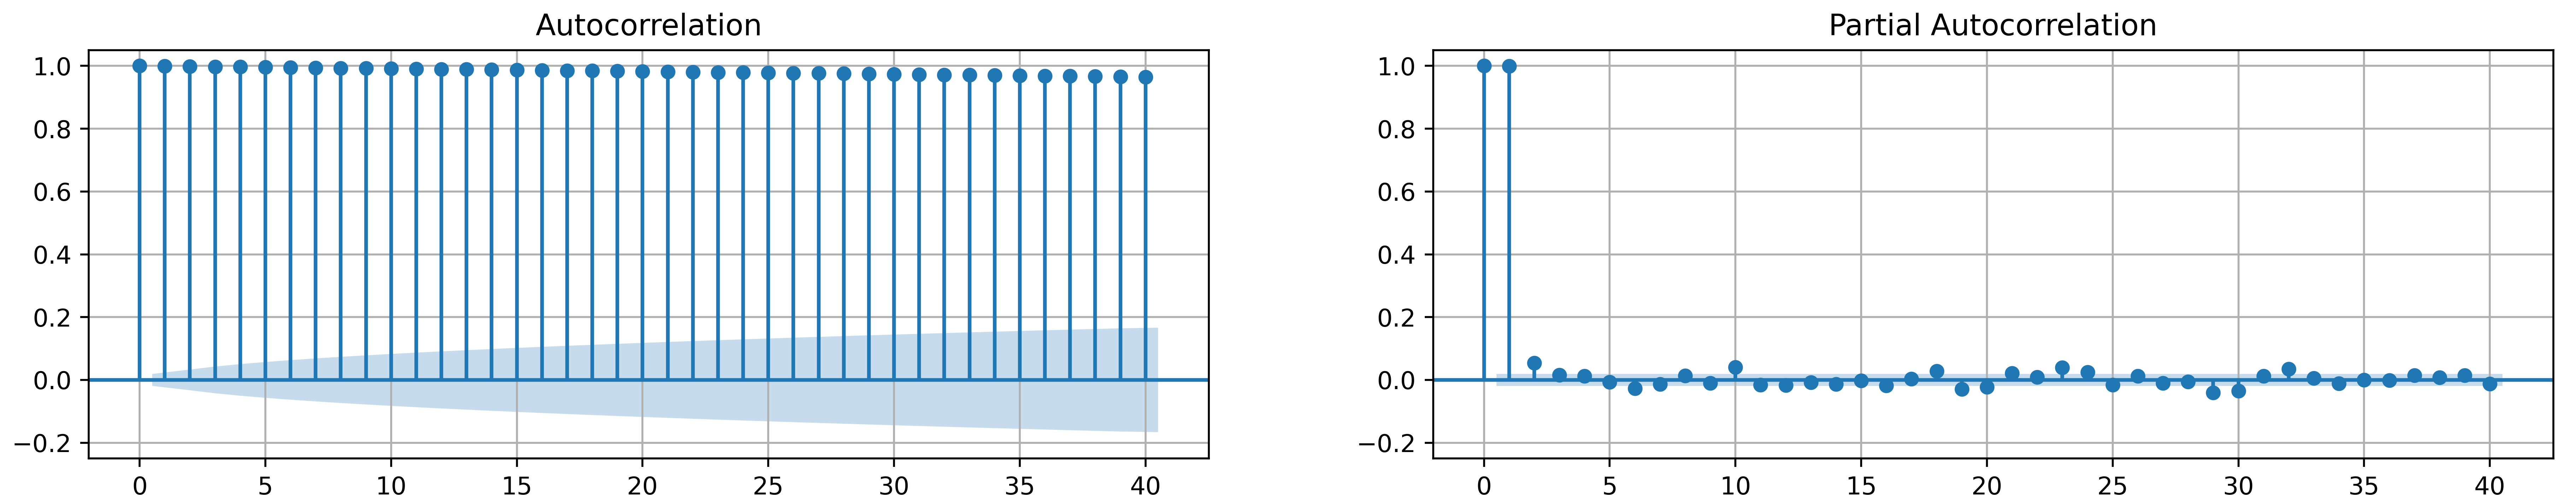
\includegraphics[width=17.5cm]{arfima/acf_pacf_for_initial_series.png}
		\caption{ACF и PACF для цены открытия акций Apple (c IPO по 2022 г)}
	\end{figure}
	Анализируя график ACF, видим, что даже 40-й лаг значим, таким образом, делается вывод, что имеющийся процесс имеет длинную память, то есть имеет смысл вычислять экспоненту Херста.
	
	\item Переходим к стационарному ряду, так как исходный, даже посредством визуального анализа не является стационарным. Более того, исходя из теста KPSS (\textbf{H0}: стационарность), стационарность ряда отвергается на 1\%-ом уровне значимости.
	\begin{figure}[H]
		\centering
		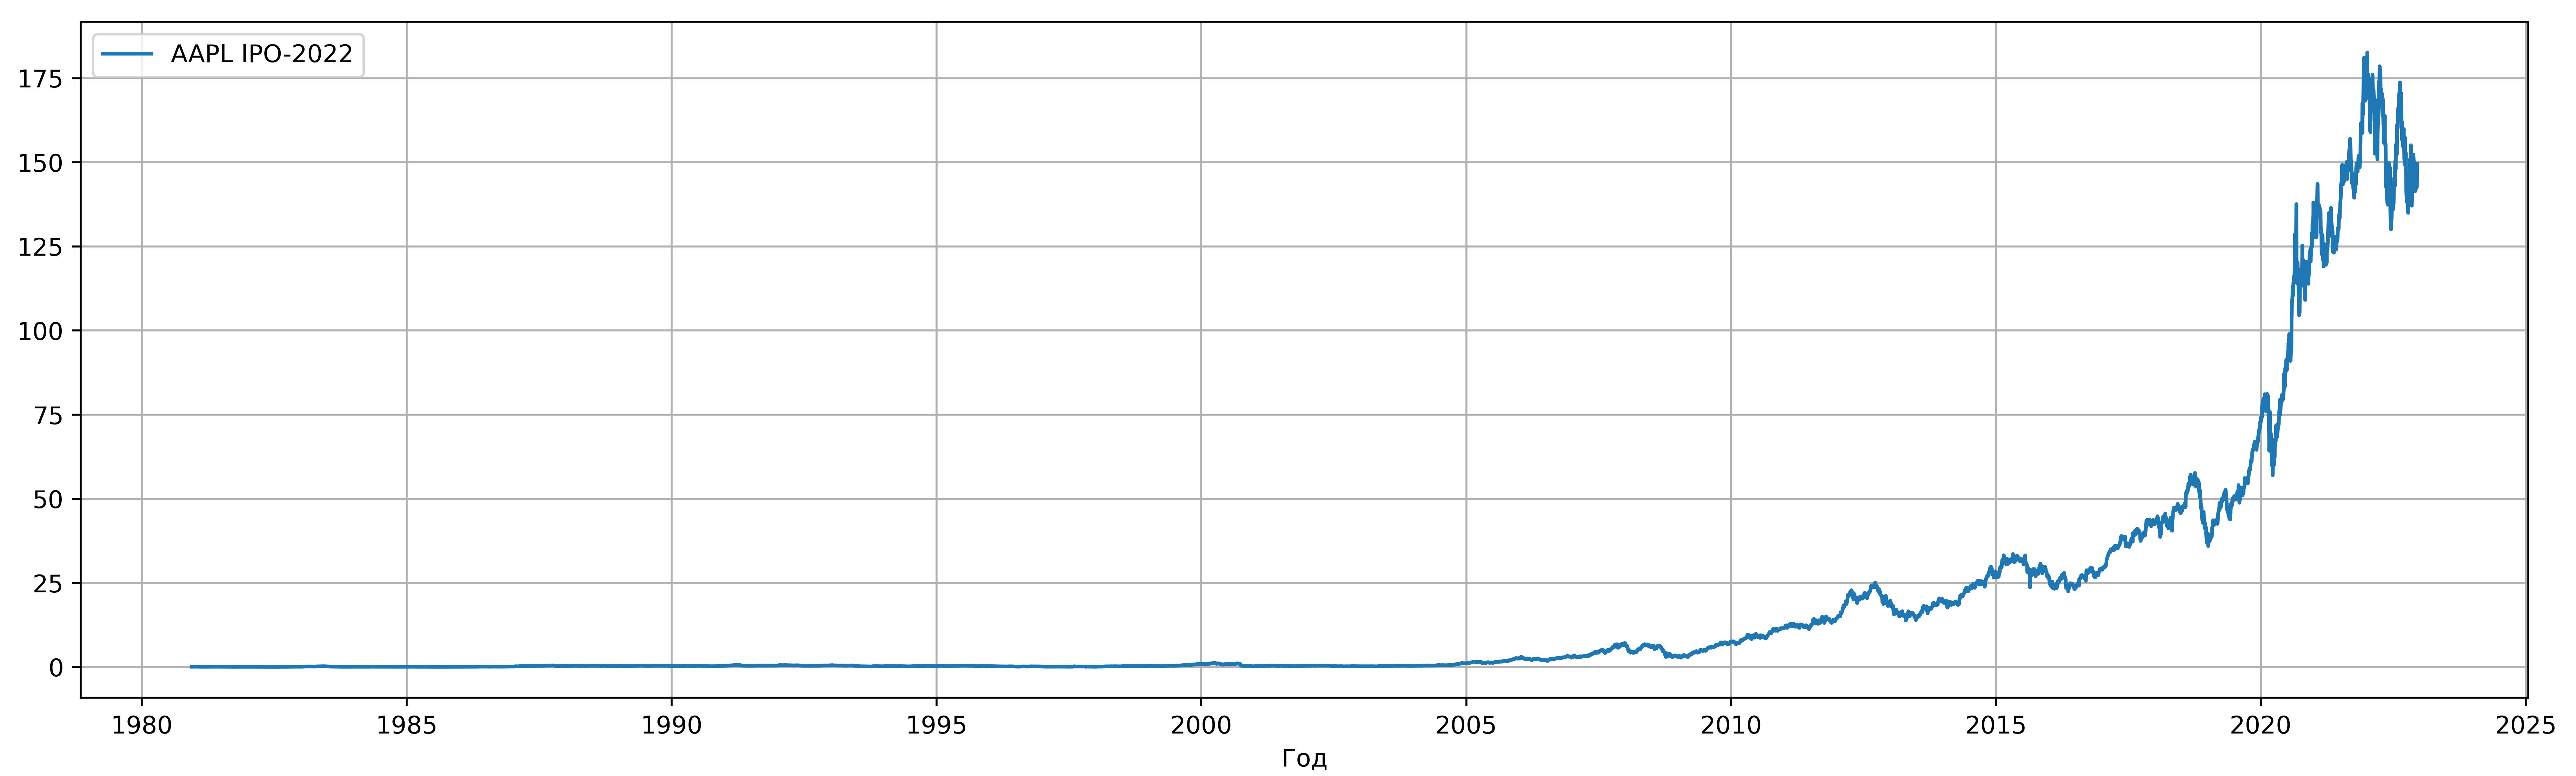
\includegraphics[width=17.5cm]{arfima/initial_ts.png}
		\caption{Цены открытия акций Apple (c IPO по 2022 г)}
	\end{figure}
	\noindent Переходим к 1-м разностям:
	\begin{figure}[H]
		\centering
		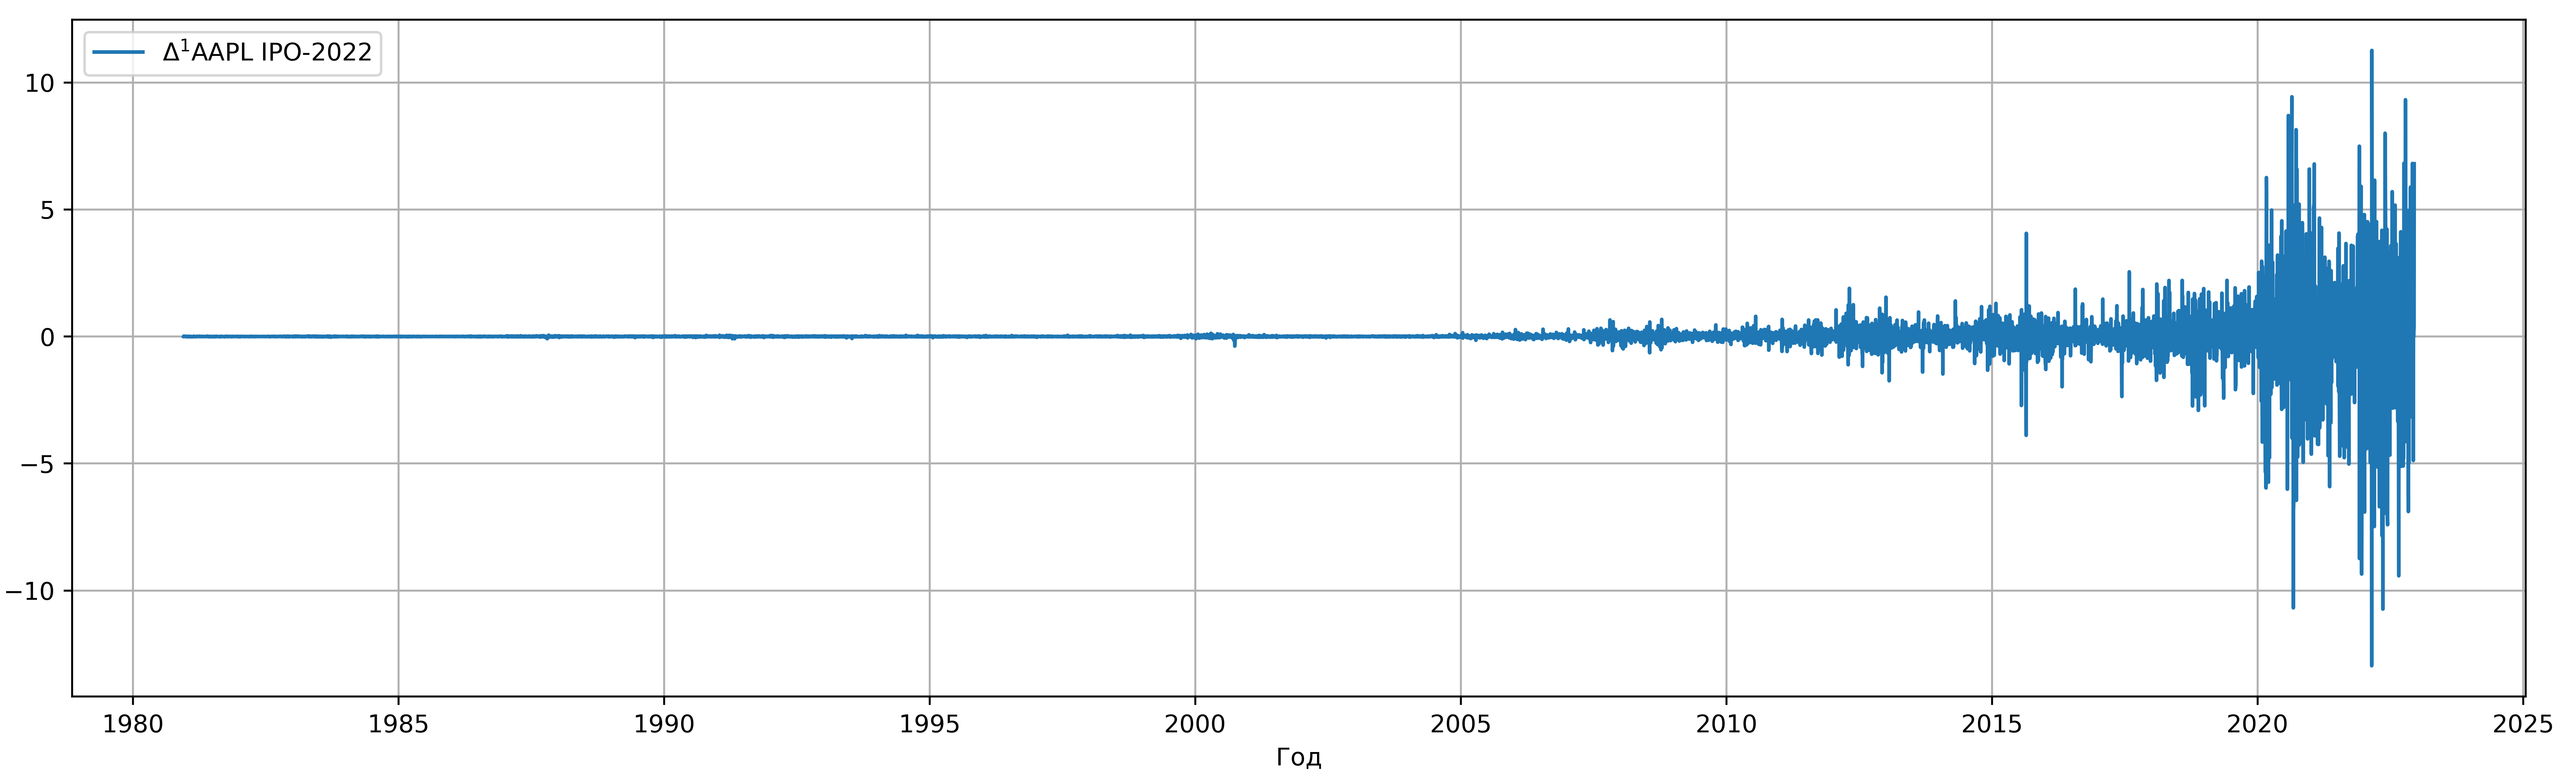
\includegraphics[width=17.5cm]{arfima/diff_1_ts.png}
		\caption{Первые разности цены открытия акций Apple (c IPO по 2022 г)}
	\end{figure}
	\noindent Посредством проведенного ADF (\textbf{H0}: нестационарность, Augmented Dicky-Fuller \cite{adf_unit_root_test}) теста, получаем безоговорочную стационарность. Даже несмотря на нестационарность первых разностей по KPSS, оставляем ряд таким, какой он есть.
	
	\item Далее оцениваем экспоненту Херста посредством применения R/S модифицированной статистики. Получаем, что значение вычисленной статистики $2.674$, что позволяет отвергнуть \textbf{H0}: наличие краткосрочной памяти на 1\%-м уровне. Таким образом, действительно, у процесса есть долгосрочная память \footnote{Результат получен при использовании пакета Gretl под названием <<\href{https://gretl.sourceforge.net/cgi-bin/gretldata.cgi?opt=SHOW_FUNCS}{ModRS\_test}>>, опубликованного в 2018 году Daniel Ventosa.} . Сама же экспонента Херста равна $0.566$, то есть, используя соотношение:
	\begin{equation}
		H = 0.5 + d
	\end{equation}
	Получаем, что порядок интегрирования ($d$) равняется приблизительно $0.066$.
	
	\item Переходим к дробно-интегрированному процессу.
	\begin{figure}[H]
		\centering
		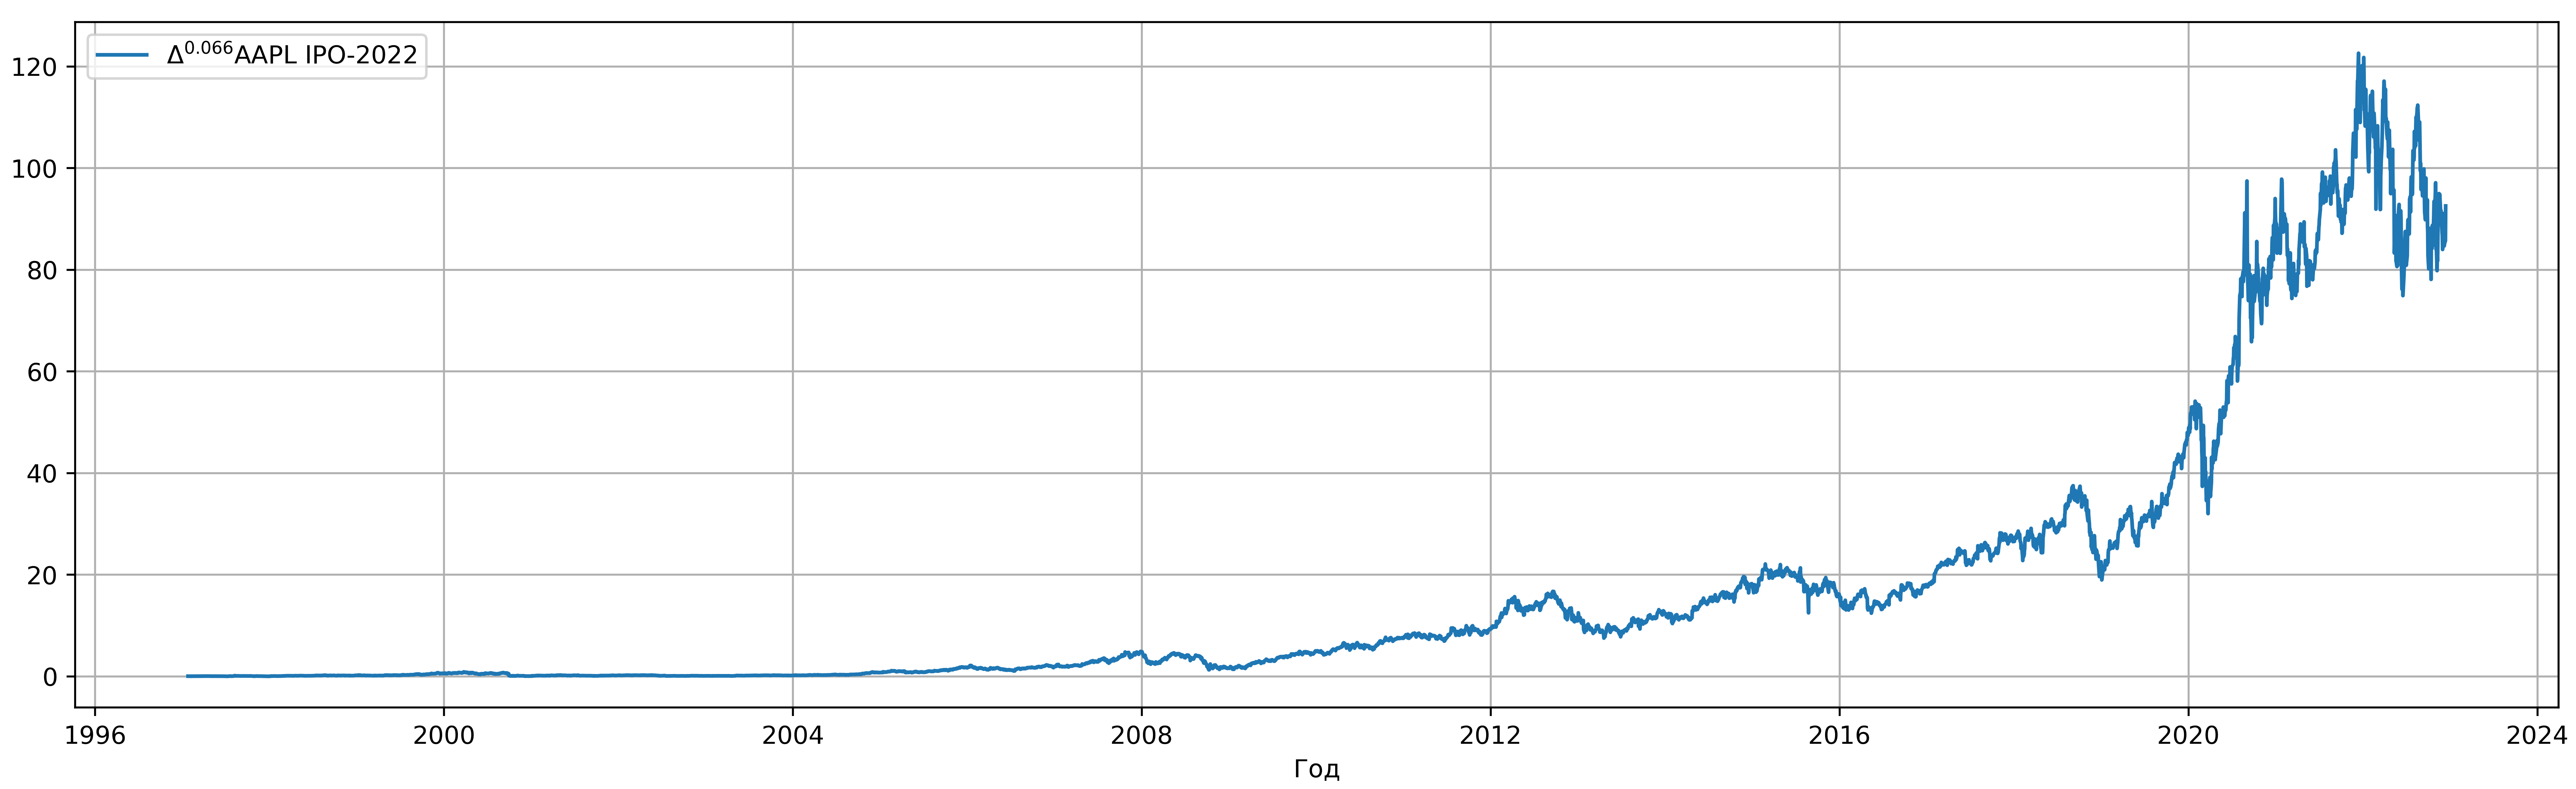
\includegraphics[width=17.5cm]{arfima/frac_diff_ts.png}
		\caption{Дробные разности цены открытия акций Apple (c IPO по 2022 г)}
	\end{figure}

	\item Далее, применяя ранее описанный алгоритм ARIMA, подбираем модель, наиболее точно описывающую полученные значения, и прогнозируем цены уже для дробно-интегрированного ряда.
	\begin{table}[H]
		\centering
		\begin{tabular}{r|ccc}
			\toprule
			Модель & \multicolumn{3}{c}{ARFIMA$(0, 1, 2)$}\\
			\midrule[0.02cm]
			Зависимая переменная & \multicolumn{3}{c}{Дробная разность Цены открытия}\\
			Количество наблюдений & \multicolumn{3}{c}{$10'561$} \\
			AIC & \multicolumn{3}{c}{$24'596$} \\
			BIC & \multicolumn{3}{c}{$24'618$} \\
			\midrule[0.02cm]
			Тест Ljung-Box (Q) & \multicolumn{2}{c}{$0.10$} & P-val ($0.75$)\\
			Тест Jarque-Bera (JB) & \multicolumn{2}{c}{$1'290'551$} & P-val ($0.00$)\\
			Тест Heteroskedasticity & \multicolumn{2}{c}{$23'355$} & P-val ($0.00$)\\
			\midrule[0.02cm]
			Первый лаг MV - $\beta_1$ & $-0.144$ & std ($0.044$) & P-val ($0.00$)\\
			Второй лаг MV - $\beta_2$ & $-0.072$ & std ($0.037$) & P-val ($0.05$)\\
			Оцененная дисперсия - $\sigma^2$ & $0.601$ & std ($0.044$) & P-val ($0.00$)\\
			\midrule[0.02cm]
		\end{tabular}
		\caption{Таблица по оценке иллюстративной модели ARFIMA$(0,1 + 0.066,2)$}
	\end{table}
	\noindent Остатки модели и их плотность распределения имеют вид:
	\begin{figure}[H]
		\centering
		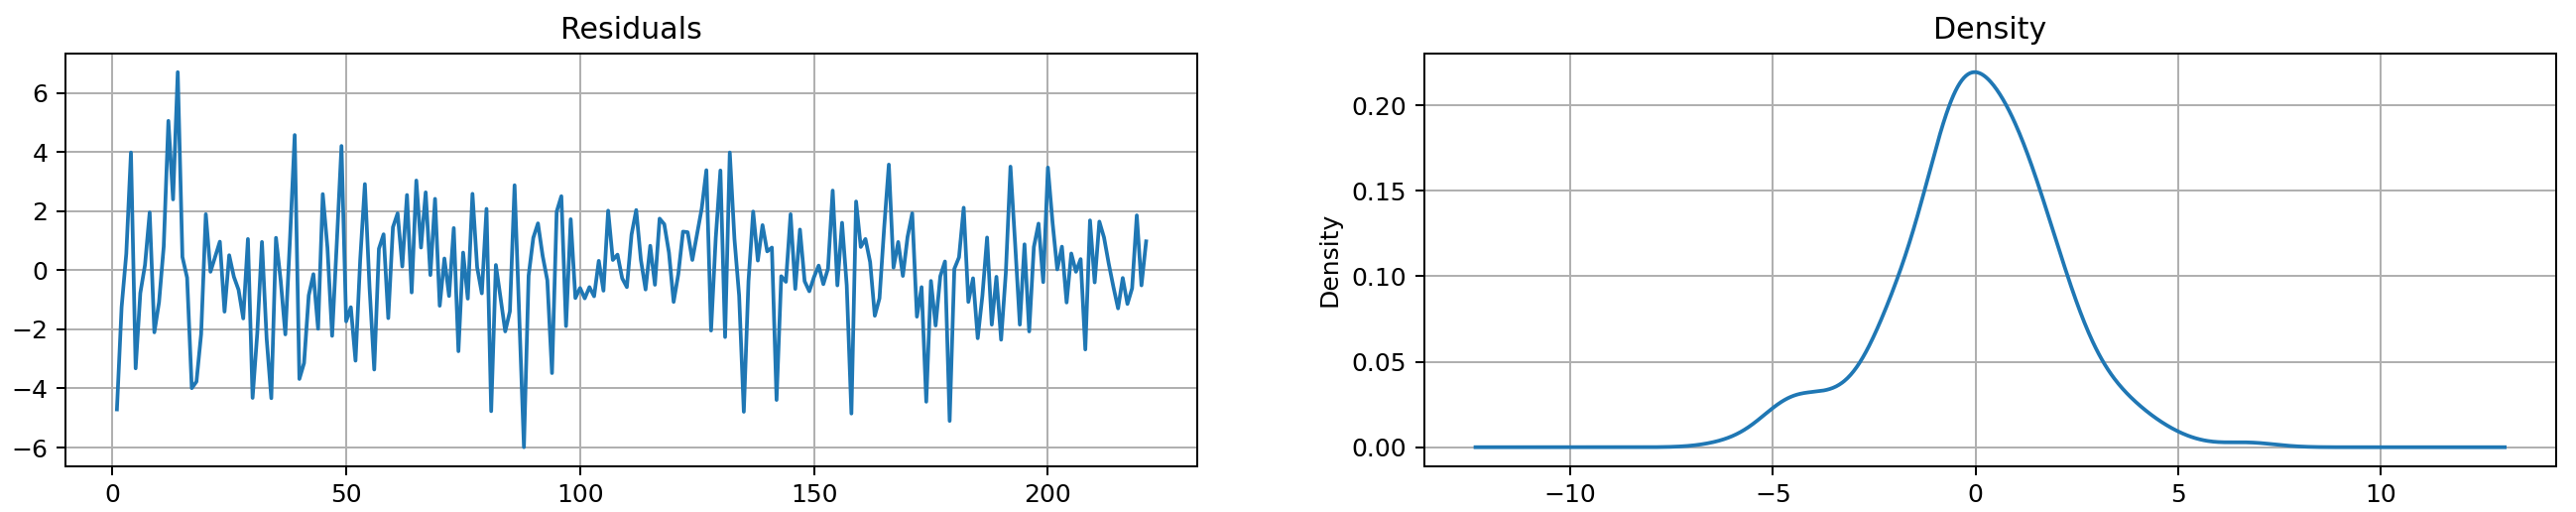
\includegraphics[width=17cm, height=4cm]{arfima/residuals_and_density.png}
		\caption{Остатки и их распределение от ARFIMA$(0, 1 + 0.066, 2)$}
	\end{figure}
	\noindent Трудно сказать, что их плотность напоминает нормальное распределение, более того сами остатки далеко не одинаковые. Подобное ухудшение в качестве предсказаний (по сравнению с ARIMA) получилось из-за того, что для модели с долгосрочной памятью необходимо очень много наблюдений, в то время как ARIMA подобного требования не выдвигает. Более того, необходимо принять особенность самих данных, ведь, глядя на график цены открытия Apple видно, что растет она экспоненциально, что заметно ухудшает способность модели корректно выдавать прогнозное значение. Далее рассматриваем автокорреляцию в остатках.
	\begin{figure}[H]
		\centering
		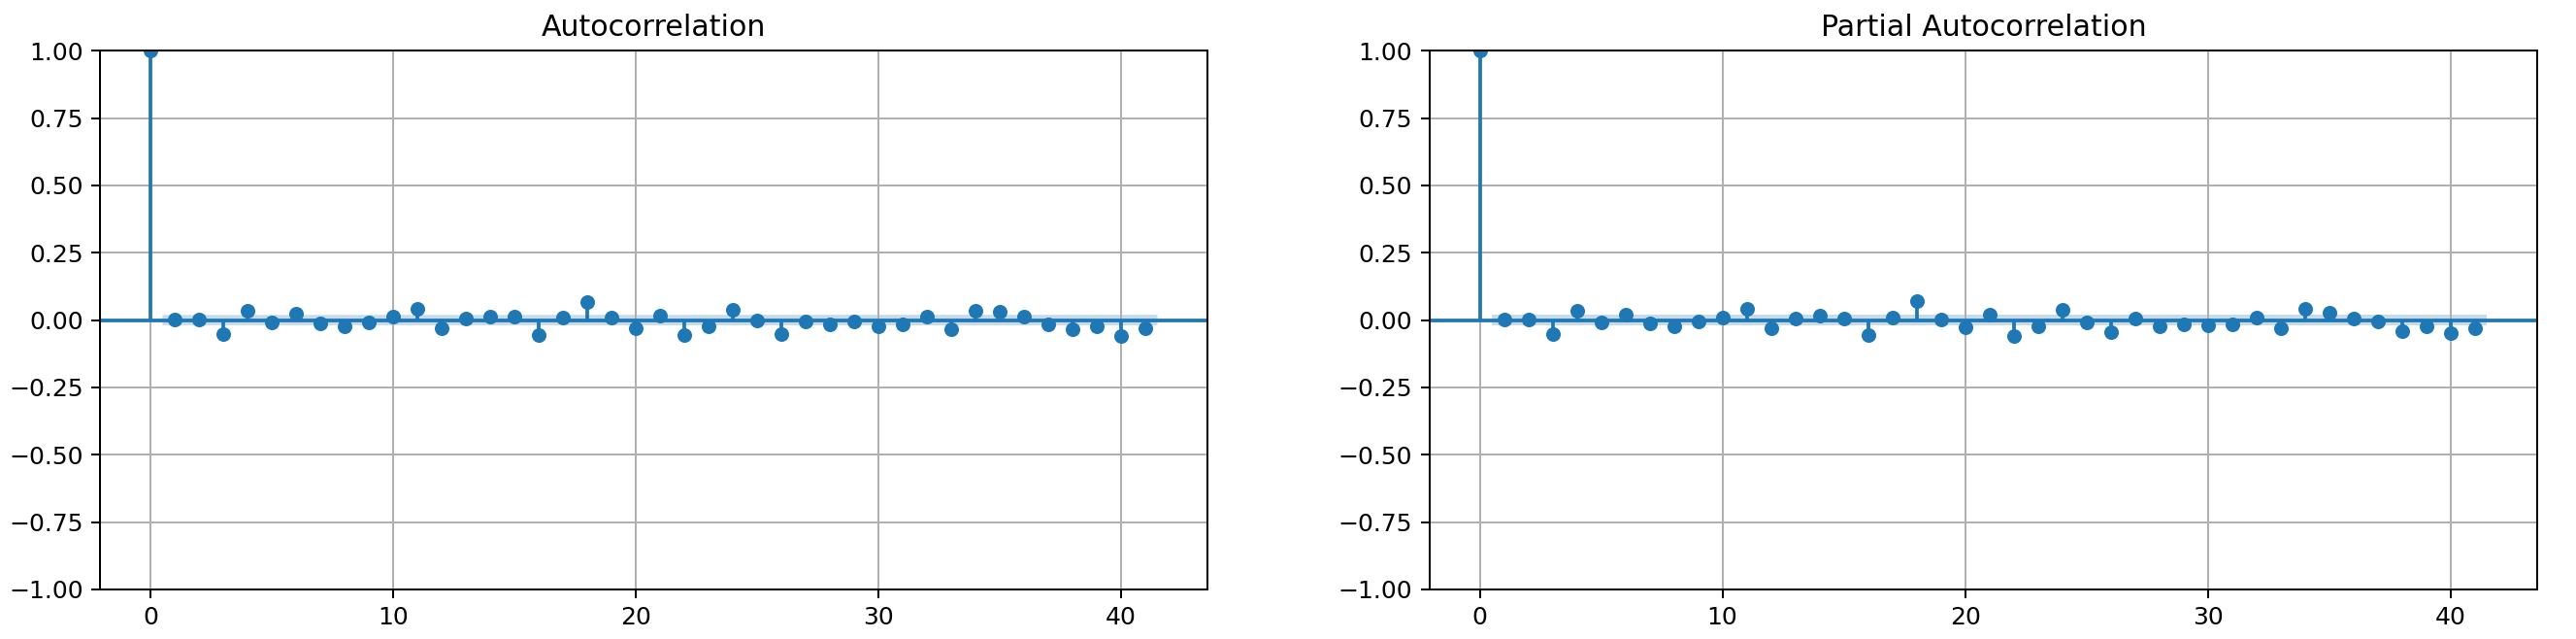
\includegraphics[width=17cm, height=4cm]{arfima/residuals_acf_pacf.png}
		\caption{ACF и PACF для остатков моделирования ARFIMA$(0, 1 + 0.66, 2)$}
	\end{figure} 
	\noindent Тут наблюдается автокорреляция, однако более высоких порядков, чем 1-2, то есть пока что отбрасываем ее. Следовательно, делаем вывод, что автокорреляции нет, даже, несмотря на то, что она есть. В итоге, пытаемся прогнозировать значения цен открытия. Хотя сразу отмечаем, что подобной малой модели трудно описать имеющиеся данный из-за их доступного количества и их особенностей соответственно.
	\begin{figure}[H]
		\centering
		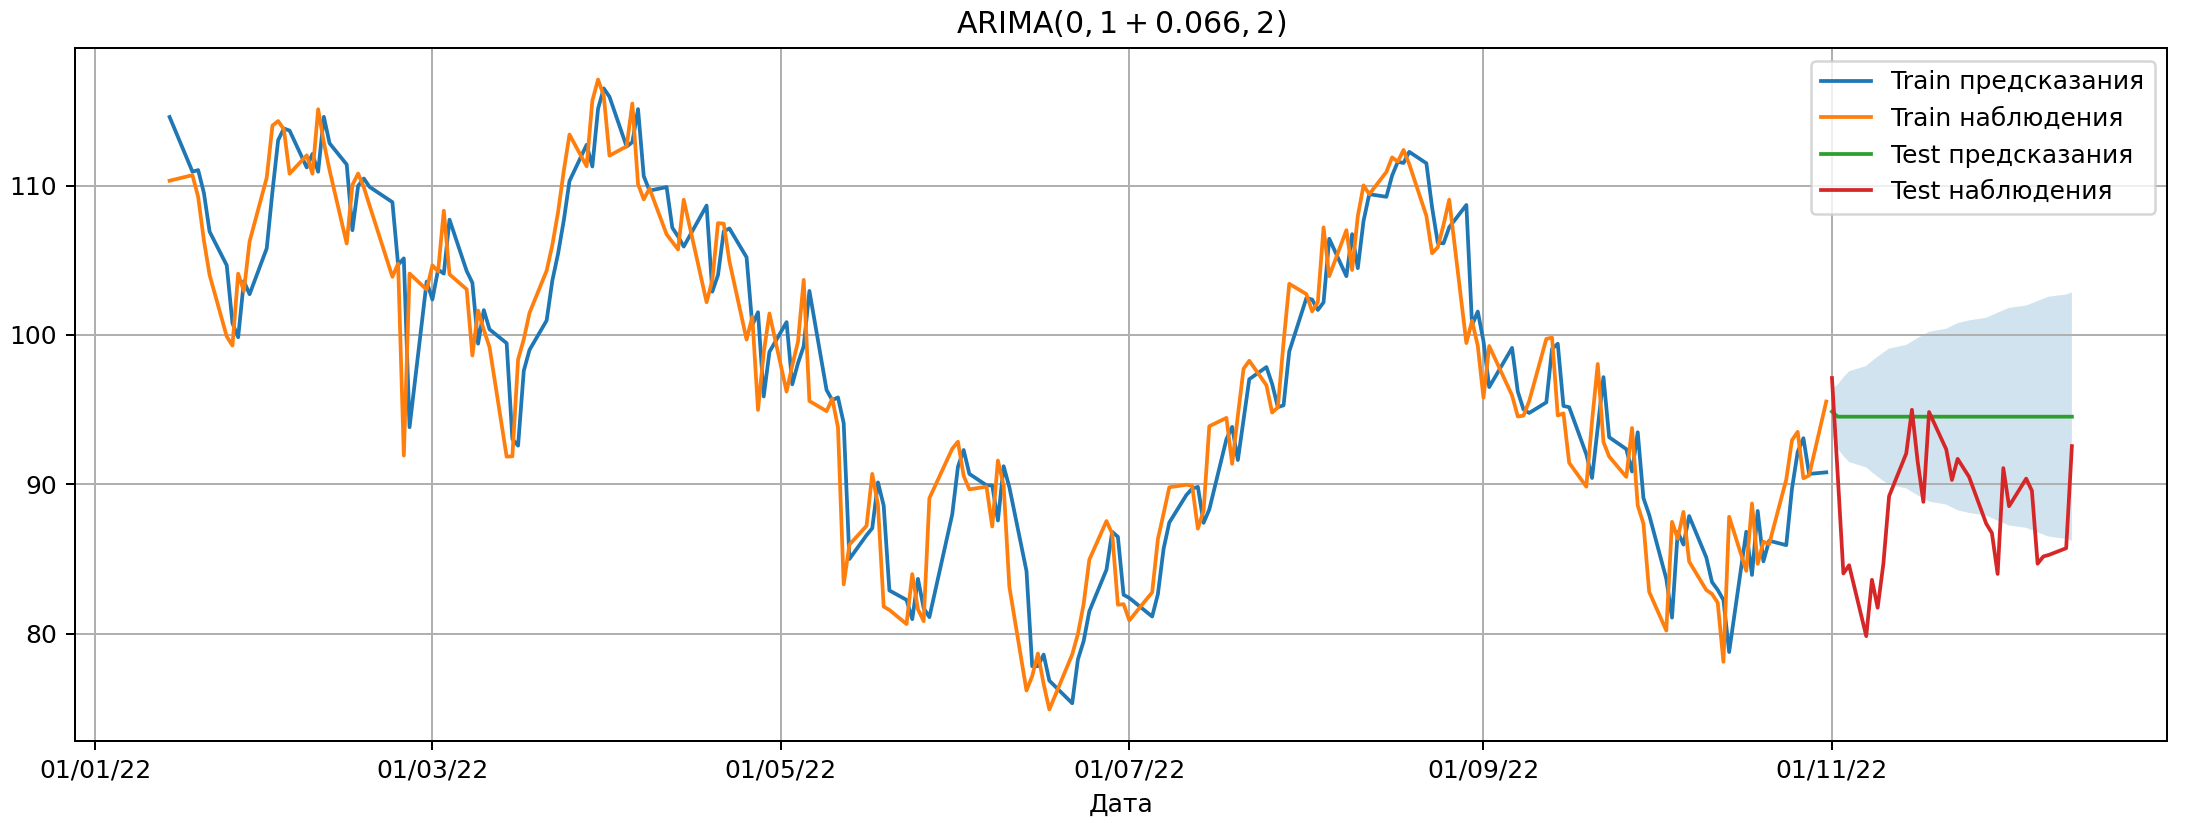
\includegraphics[width=17cm, height=6.25cm]{arfima/final_picture.png}
		\caption{Моделирование предсказаний посредством модели}
	\end{figure}
\end{enumerate}
\noindent Вывод таков, что настоящая модель не может корректно обработать, то есть обучиться на предоставленных данных, несмотря на оправдывающую себя математику теории фракталов, стоящую за ней (моделью). Напоминаю, что подобное произошло не из-за низкого качества модели, а из-за поведения цен открытия Apple. То есть, конечно, данная модель участвует в формировании финальной сравнительной таблицы, однако берем на заметку, что для Apple лучше использовать комбинацию авторегрессионных моделей и моделей, описывающий условную гетероскедастичность: ARCH, GARCH, FIGARCH. Так как волатильность цены открытия, исходя из графика остатков, увеличивается все больше и больше под конец наблюдаемых значений.